\documentclass[journal]{IEEEtran}
\usepackage{amsmath,amsfonts}
\usepackage{algorithmic}
\usepackage{algorithm}
\usepackage{array}
\usepackage[caption=false,font=normalsize,labelfont=sf,textfont=sf]{subfig}
\usepackage{textcomp}
\usepackage{stfloats}
\usepackage{url}
\usepackage{verbatim}
\usepackage{graphicx}
\usepackage{cite}

\usepackage{makecell, tabularx}
\usepackage{tabularx}
\usepackage{amsmath}
\usepackage{amsfonts}
\usepackage{tikz}
\usepackage{multirow}
\usepackage{xcolor}
\usepackage[export]{adjustbox}

\hyphenation{op-tical net-works semi-conduc-tor IEEE-Xplore}
% updated with editorial comments 8/9/2021

\begin{document}

\title{Beyond Subspace Isolation: \\ Many-to-Many Transformer for Light Field Image Super-resolution}

\author{Zeke Zexi Hu, Xiaoming Chen,~\IEEEmembership{Member, IEEE}, Vera Yuk Ying Chung,~\IEEEmembership{Member, IEEE}, Yiran Shen,~\IEEEmembership{Senior Member, IEEE}
\thanks{Zeke Zexi Hu and Vera Yuk Ying Chung are with the School of Computer Science, University of Sydney, Darlington, NSW 2008, Australia.}
\thanks{Xiaoming Chen is with the School of Computer Science and Engineering, Beijing Technology and Business University, Beijing 102488, China.}
\thanks{Yiran Shen is with the School of Software, Shandong University, Jinan, 250100, China.}
}

% The paper headers
\markboth{Journal of \LaTeX\ Class Files,~Vol.~14, No.~8, August~2021}%
{Shell \MakeLowercase{\textit{et al.}}: A Sample Article Using IEEEtran.cls for IEEE Journals}

% \IEEEpubid{0000--0000/00\$00.00~\copyright~2021 IEEE}
% Remember, if you use this you must call \IEEEpubidadjcol in the second
% column for its text to clear the IEEEpubid mark.

\maketitle

\begin{abstract}
    The effective extraction of spatial-angular features plays a crucial role in light field image super-resolution (LFSR) tasks, and the introduction of convolution and Transformers leads to significant improvement in this area. Nevertheless, due to the large 4D data volume of light field images, many existing methods opted to decompose the data into a number of lower-dimensional subspaces and perform Transformers in each sub-space individually. As a side effect, these methods inadvertently restrict the self-attention mechanisms to a One-to-One scheme accessing only a limited subset of LF data, explicitly preventing comprehensive optimization on all spatial and angular cues. In this paper, we identify this limitation as subspace isolation and introduce a novel Many-to-Many Transformer (M2MT) to address it. M2MT aggregates angular information in the spatial subspace before performing the self-attention mechanism. It enables complete access to all information across all sub-aperture images (SAIs) in a light field image. Consequently, M2MT is enabled to comprehensively capture long-range correlation dependencies. With M2MT as the pivotal component, we develop a simple yet effective M2MT network for LFSR. Our experimental results demonstrate that M2MT achieves state-of-the-art performance across various public datasets. We further conduct in-depth analysis using local attribution maps (LAM) to obtain visual interpretability, and the results validate that M2MT is empowered with a truly non-local context in both spatial and angular subspaces to mitigate subspace isolation and acquire effective spatial-angular representation. 
\end{abstract}

\begin{IEEEkeywords}
Light field, Super-resolution, Image processing, Deep learning.
\end{IEEEkeywords}

\section{Introduction} \label{section:Introduction}

Light field (LF) images, unlike regular images captured by monocular cameras, provide richer information by capturing light rays from multiple angular directions in a single shot. This unique characteristic has paved the way for substantial progress in various computer vision applications where conventional cameras have shown limited efficacy, \textit{e.g.,} material recognition \cite{wangLFRecognition_ECCV2016, luLFRecognition_2019}, depth estimation \cite{yucer2016efficient, heberUshapeICCV2017, wangOcclusionawareDepthEstimation2015, chaoSubFocal_TCI2023, ding_TCI2023}, salient object detection under complex scenarios \cite{shengLFSaliency_ICASSP2016, zhangLFNet_TIP2020, chen_TMM2023}, microsopy \cite{verinaz_TCI2022, verinaz_TCI2023, levoy2006light}, and anti-spoof face recognition \cite{raghavendraLFFace_TIP2015, jiLFHOG_ICIP2016}. By simultaneously capturing multiple sub-aperture images (SAIs, or views), LF technology enables a rich and interactive viewing experience. Users can freely explore and interact with the virtual environments, changing perspectives and moving within them. Therefore, LF technology has become a cornerstone of VR applications, enhancing user engagement and immersion.


\newcommand{\imageWithGrid}[3]{%
  \begin{tikzpicture}
    \node[anchor=south west,inner sep=0] (image) at (0,0) {\includegraphics[width=#2, height=#3]{#1}};
    \begin{scope}[x={(image.south east)},y={(image.north west)}]
        \foreach \i in {1,...,4} {
            \draw[lightgray,thin] (\i/5,0) -- (\i/5,1); % Vertical lines
            \draw[lightgray,thin] (0,\i/5) -- (1,\i/5); % Horizontal lines
        }
        \draw[black] (0,0) rectangle (1,1);
    \end{scope}
  \end{tikzpicture}%
}


\begin{figure}[t!]
\centering

\tabcolsep=0.04cm
\renewcommand{\arraystretch}{0.8}
\begin{tabular}{ccccc}
    \raisebox{0.5\height}{
        \resizebox{0.05\textwidth}{!}{
        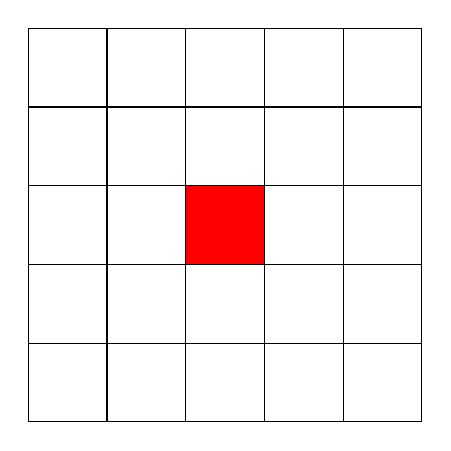
\begin{tikzpicture}
            \foreach \x in {0,1,2,3,4} {
                \foreach \y in {0,1,2,3,4} {
                    \draw[black, thin] (\x,\y) rectangle (\x+1,\y+1);
                }
            }
            \draw[black] (0,0) rectangle (5,5);
            \fill[red] (2,2) rectangle (3,3);
        \end{tikzpicture}}
    } &
    \includegraphics[width=0.09\textwidth]{img/qual/Perforated_Metal_3/LR.annotated.png} &
    \includegraphics[width=0.09\textwidth]{img/qual/Perforated_Metal_3/EPIT/SR.png} &
    \includegraphics[width=0.09\textwidth]{img/qual/Perforated_Metal_3/SAT/SR.png} &
    \includegraphics[width=0.09\textwidth]{img/qual/Perforated_Metal_3/HR.png} \\
    \footnotesize{\makecell{SAI\\Location}} & \footnotesize LR & \footnotesize EPIT & \footnotesize M2MT-Net & \footnotesize HR
\end{tabular} \\

(a) SAI location and patch images. \\
\hspace{0pt}

\tabcolsep=0.1cm
\begin{tabular}{cc}
    \imageWithGrid{img/qual/Perforated_Metal_3/EPIT/LAM.png}{0.18\textwidth}{0.18\textwidth} &
    \imageWithGrid{img/qual/Perforated_Metal_3/SAT/LAM.png}{0.18\textwidth}{0.18\textwidth} \\
    % \includegraphics[width=0.22\textwidth,cfbox=black 0.5pt 0pt]{img/qual/Perforated_Metal_3/EPIT/LAM.png} &
    % \includegraphics[width=0.22\textwidth,cfbox=black 0.5pt 0pt]{img/qual/Perforated_Metal_3/SAT/LAM.png} \\
    EPIT (DI: 5.9518) & M2MT (DI: 27.2578) \\
\end{tabular} \\
\vspace{8pt}
(b) Local attribution maps of SAIs: Diffusion Index (DI) quantifies the extent of influential pixels.\\
% From the original paper: The Diffusion Index (DI) reflects the range of involved pixels. A higher DI represents a wider range of attention.
%DI represents Diffusion Index.\\
\hspace{0pt}
\caption{Super-resolved results and local attribute maps (LAM) of the proposed M2MT-Net against the current state-of-the-art methods on the \textit{Perforated\_metal\_3} sample.}
% \caption{Illustration of super-resolved images and LAM comparing EPIT and M2MT on a patch of the \textit{Perforated metal 3} sample.}

\label{fig:First}
\end{figure}


Capturing LF images necessitated self-built dense camera arrays \cite{wilburn2004high, wilburn2005high}, which were prohibitively expensive and not ready for mainstream use. However, advancements of sophisticated LF cameras like Raytrix \cite{Raytrix}, Lytro Illum \cite{Lytro}, and Google's Light Field VR Camera \cite{GoogleLF} have gradually democratized LF imaging, making it accessible for both commercial and industrial applications. Despite this progress, LF cameras have long faced the challenges in striking a balance angular and spatial resolutions due to inherent limitations in sensor capabilities, often leading to lower spatial resolutions compared to traditional cameras.

Researchers have developed a number of possible solutions and they generally fall into two categories: light field image super-resolution (LFSR) \cite{yeungSAS_LFSR2019,wangDistgSSR_TIP2022} and light field angular super-resolution (also known as light field view synthesis) \cite{liu_TMM2022, yeungSAS_ECCV2018}. LFSR aims to upsample the spatial resolution of each SAI, effectively reconstructing the details within the views, which is the focus of this paper. On the other hand, light field angular super-resolution focuses on synthesizing additional SAIs to enhance the angular resolution of the light field. This paper primarily concentrates on LFSR.

\begin{figure*}[t!]
    \definecolor{myred}{HTML}{FF0080}
    \definecolor{myblue}{HTML}{007FFF}
    \centering

    \tabcolsep=0.10cm
    \renewcommand{\arraystretch}{0.1}
    \setlength{\medmuskip}{-1mu}
    \begin{tabular}{cc}
        \raisebox{0.025\height}{
        \includegraphics[width=0.250\linewidth]{img/cubes/LF.pdf}
        }
        &
        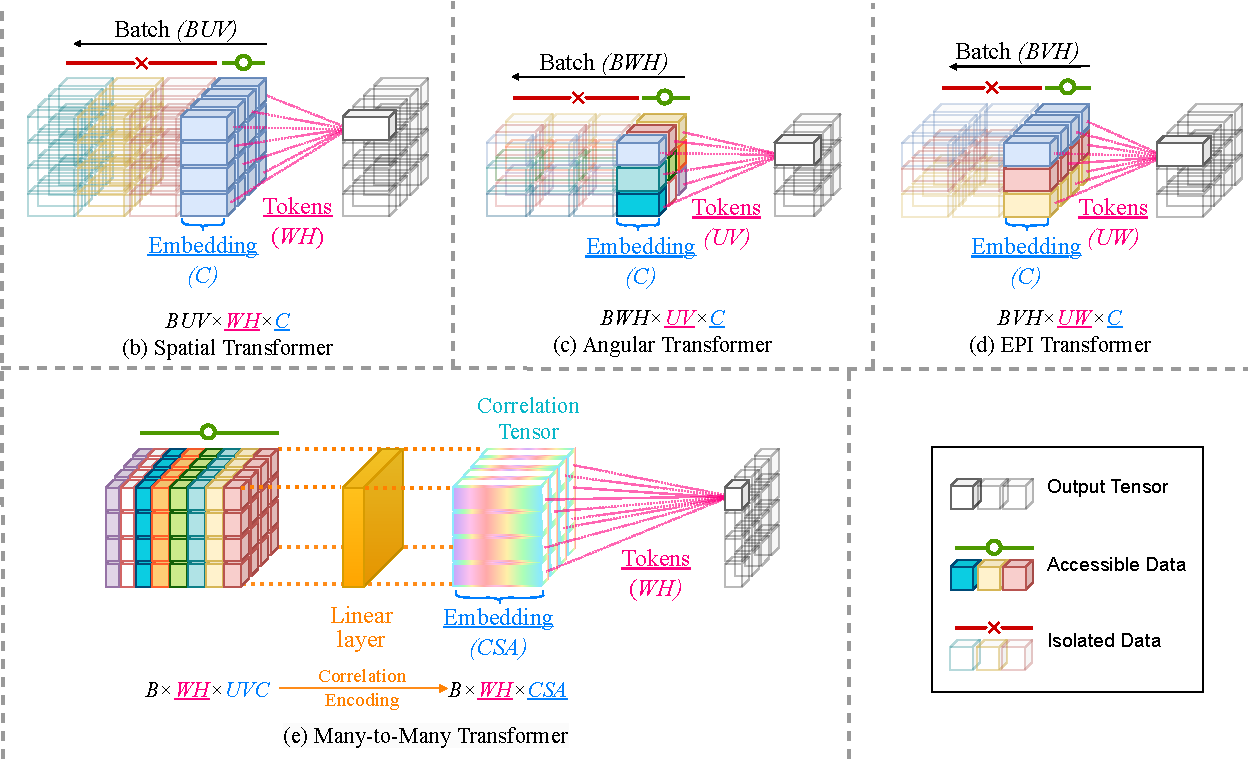
\includegraphics[width=0.660\linewidth]{img/cubes/main.pdf}
        % \begin{tabular}{ccc}
        %     \includegraphics[height=0.155\linewidth]{img/cubes/Spatial.pdf} &
        %     \includegraphics[height=0.155\linewidth]{img/cubes/Angular.pdf} &
        %     \includegraphics[height=0.155\linewidth]{img/cubes/EPI.pdf} \\
        %     \footnotesize $BU\!V \times \textcolor{myred}{\underline{W\!H}} \times \textcolor{myblue}{\underline{C}}$ &
        %     \footnotesize $BW\!H \times \textcolor{myred}{\underline{U\!V}} \times \textcolor{myblue}{\underline{C}}$ &
        %     \footnotesize $BV\!H \times \textcolor{myred}{\underline{U\!W}} \times \textcolor{myblue}{\underline{C}}$ \\
        %     \footnotesize (b) Spatial Transformer. &
        %     \footnotesize (c) Angular Transformer. &
        %     \footnotesize (d) EPI Transformer. \\
        %     \vspace{0pt} & \\
        %     \multicolumn{3}{c}{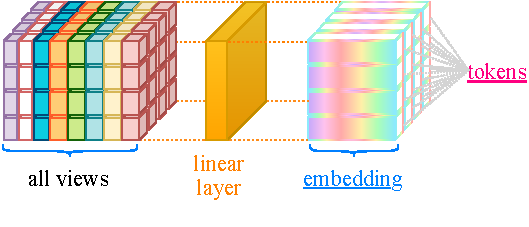
\includegraphics[height=0.18\linewidth]{img/cubes/SAT.pdf}} \vspace{-8pt} \\
        %     \multicolumn{3}{c}{\footnotesize $B \times \textcolor{myred}{\underline{W\!H}} \times \textcolor{myblue}{\underline{C_{SA}}}$} \\
        %     \multicolumn{3}{c}{\footnotesize (e) Spatial-angular Transformer.} \\
        % \end{tabular}
    \end{tabular}

    % \tabcolsep=0.20cm
    % \renewcommand{\arraystretch}{1}
    % \setlength{\medmuskip}{-1mu}
    % \begin{tabular}{ccccc}
    %     \includegraphics[width=0.1\linewidth]{img/cubes/LF.pdf} &
    %     \includegraphics[width=0.2\linewidth]{img/cubes/Spatial.pdf} &
    %     \includegraphics[width=0.2\linewidth]{img/cubes/Angular.pdf} &
    %     \includegraphics[width=0.2\linewidth]{img/cubes/EPI.pdf} &
    %     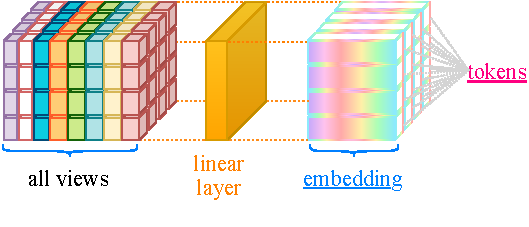
\includegraphics[width=0.2\linewidth]{img/cubes/SAT.pdf} \\
    %     \makecell{
    %         \footnotesize $U \times V \times W \times H \times C$ \\
    %         \footnotesize (a) LF image and tensor.
    %     } &
    %     \makecell{
    %         \footnotesize $U\!V \times \textcolor{myred}{\underline{W\!H}} \times \textcolor{myblue}{\underline{C}}$ \\
    %         \footnotesize (b) Spatial transformer. \\
    %     } &
    %     \makecell{
    %         \footnotesize $W\!H \times \textcolor{myred}{\underline{U\!V}} \times \textcolor{myblue}{\underline{C}}$ \\
    %         \footnotesize (c) Angular transformer. \\
    %     } &
    %     \makecell{
    %         \footnotesize $V\!H \times \textcolor{myred}{\underline{U\!W}} \times \textcolor{myblue}{\underline{C}}$ \\
    %         \footnotesize (d) EPI transformer. \\
    %     } &
    %     \makecell{
    %         \footnotesize $V\!H \times \textcolor{myred}{\underline{U\!W}} \times \textcolor{myblue}{\underline{C}}$ \\
    %         \footnotesize (e) Spatial-angular transformer. \\
    %     }
    % \end{tabular}
    \caption{Illustration of available data in LF tensors used by existing LF Transformers under the One-to-One scheme and our proposed Many-to-Many Transformer. For the tensors, each color represents a SAI.}
    \label{fig:Cubes}
\end{figure*}


\noindent{\bf Motivations.} The advances in deep learning, particularly convolutional neural networks (CNNs) \cite{yoon2017LFCNN, yeungSAS_LFSR2019, wangDistgSSR_TIP2022} and Vision Transformers (ViT) \cite{dosovitskiyViT_arXiv2020, liuSwin_ICCV2021, luESRT_CVPR2022}, have led to significant improvement in LFSR than traditional methods \cite{wanner2014variational}. The success has also extended to LFSR by processing 4D LF images in 2D subspaces, such as spatial, angular \cite{wangDPT_AAAI2022, liangLFT_SPL2022}, or Epipolar Image (EPI) \cite{liangEPIT_arXiv2023} subspaces. However, these methods predominantly suffer from subspace isolation, a defect causing sub-optimal performance.

Specifically, this issue arises when adapting 2D operations to the 4D LF data, existing approaches have to compromise its complete access to the LF information. This is primarily because training networks directly on voluminous 4D LF data, e.g. 4D convolutions \cite{yeungSAS_LFSR2019}, demands a relatively large number of weights, which is prone to optimization difficulties and heavy computation. As a workaround, most previous methods decompose the 4D data into 2D subspaces such as spatial and angular subspaces, or EPI subspaces. In implementation, one typical practice is to temporarily reshape a 4D tensor to expose two operative dimensions as tokens while merging the other two dimensions with the batch dimension. This decomposition enables 2D operations to perform on 4D LF tensors, and in training, the optimization is conducted on the whole tensor. However, a significant limitation arises during inference. When inferring the value at a specific location, access to the two merged dimensions is confined to only one location at a time, rather than spanning the entire dimensionality. As a result, even if with non-local Transformers, the effective receptive field is virtually restricted to a local context within the operative subspaces, leading to an One-to-One scheme.

For instance, consider the scenario depicted in Figure \ref{fig:Cubes}(a), where a single 4D LF tensor $I(u, v, x, y) \in \mathbb{R}^{U \times V \times W \times H \times C}$ is part of a batch $B$. Here, $(u, v, x, y)$ denotes a pixel's spatial location $(x, y)$ and angular location (or SAI) $(u, v)$. By merging the angular subspace $(U, V)$ into the batch dimension, a 2D spatial Transformer in Figure \ref{fig:Cubes}(b) is enabled to operate on the flatten spatial subspace $(W, H)$ as tokens across SAIs. However, this merging effectively isolates the network's forward propagation in the merged angular subspace $BUV$, as depicted by transparent blocks in the batch dimension. Consequently, the network is restricted to accessing only one SAI at a time during processing. This procedural constraint can be formally expressed as
\begin{equation} \label{eq:before}
\begin{split}
    I_{2}(u, v, x, y) = F \cdot \{I_{1}(\bar{u}, \bar{v}, \bar{x}, \bar{y})\}_{(\bar{u}, \bar{v}) = (u, v), (\bar{x}, \bar{y}) \in \mathbb{R}^{W \times H}}
    % I_{2}(u, v, x, y) = F({ \{I_{1}(u', v', x', y')\} }), & \quad (u', v') = (u, v) \\
    % & \quad (x', y') \in \mathbb{R}^{W \times H} \\
\end{split}
\end{equation}
where $F$ is a 2D operation, which can be either convolution or Transformers, and $I_{1}$ and $I_{2}$ are the input and output LF tensors of the operation. Under this scheme, to obtain a complete LF tensor, Equation \ref{eq:before} is repeated $U \times V$ times, each effectively being a One-to-One operation mapping from a SAI in $I_{1}$ at a single angular location $(u, v)$ to a SAI in $I_{2}$ at the same isolated angular location $(u, v)$ in the output. However, the ideal processing would instead use all SAIs to inform the computation loosening the constraint $(\bar{u}, \bar{v}) = (u, v)$, resulting in:
\begin{equation} \label{eq:after}
\begin{split}
    I_{2}(u, v, x, y) = F \cdot \{I_{1}(\bar{u}, \bar{v}, \bar{x}, \bar{y})\}_{(\bar{u}, \bar{v}, \bar{x}, \bar{y}) \in \mathbb{R}^{U \times V \times W \times H}}
\end{split}
\end{equation}

Subspace isolation is not unique to spatial Transformers and extends to other forms of data decomposition under the One-to-One scheme. For example, an angular Transformer is limited to accessing only one pixel across SAIs as depicted in Figure \ref{fig:Cubes}(c). Similarly, an EPI Transformer can only access a slice of two dimensions in the EPI subspace merged with the batch dimension, as shown in Figure \ref{fig:Cubes}(d). These constraints, inherent in the One-to-One operational scheme, significantly impede the ability of existing models to fully exploit the spatial and angular cues available in LF data, resulting in an incomplete spatial-angular representation.

\noindent{\bf Contributions.}
To address this issue, in this paper, we propose the novel Many-to-Many Transformer (M2MT), a new scheme to achieve the goal of comprehensive data integration outlined in Equation \ref{eq:after} and alleviate the isolation. The M2MT method begins by constructing correlation embeddings in the angular subspace. It then applies a self-attention mechanism to model long-range dependencies within the spatial subspace. This innovative approach allows the M2MT to access all the spatial and angular cues present in an LF image during each step of data propagation, thereby facilitating the creation of a holistic spatial-angular representation with a truly non-local context.

With M2MT as a foundational component, we present a simple yet effective network, M2MT-Net, incorporating M2MT in the spatial subspace and vanilla Transformers in the angular subspace. Through extensive experimental evaluation, we showcase M2MT-Net's outstanding performance, establishing it as a new state-of-the-art for LFSR.

Furthering the research, we delve into a series of analysis to discover the mechanisms behind its success. Particularly, by leveraging the technique of local attribution maps (LAM) \cite{guLAM_CVPR2021}, which visualize influential pixels, to gain interpretability of neural networks. Figure \ref{fig:First} reveals that M2MT utilizes more pixels across broader SAIs than the current state-of-the-art methods like EPIT \cite{liangEPIT_arXiv2023}. This observation substantiates the efficacy of M2MT, which mitigates the limitation of subspace isolation, simultaneously preserving more high-frequency cues in the spatial subspace and establishing a richer and non-local interplay of SAI dependencies in the angular subspace.

The contributions of this paper can be summarized as follows:
\begin{enumerate}
    \item The limitation of subspace isolation is identified, which predominantly impedes the performance of existing LF image processing methods by restricting data access when decomposing a 4D operation into a few One-to-One 2D operations.
    \item To overcome the limitations imposed by the One-to-One scheme, we introduce the Many-to-Many Transformer (M2MT), which aggregates correlation information from the angular subspace and performs a self-attention mechanism in the spatial subspace. A simple-yet-effective network, M2MT-Net, is developed incorporating the proposed M2MT for LFSR.
    \item Experimental results validate that M2MT-Net achieves state-of-the-art performance. In-depth analysis, especially the LAM analysis, is conducted to reveal its truly non-local context, utilizing all available information in a LF image for superior performance.
\end{enumerate}
\section{Related Works}
\subsection{Single Image Super-resolution}
Single Image Super-resolution (SISR) is a classic low-level computer vision task aiming to reconstruct a high-resolution image (HR) from the low-resolution (LR) counterpart. Dong et al. \cite{dongSRCNN_ECCV2014} pioneered the introduction of CNN to this task, setting a new standard that outperformed previous SISR methods. This innovation marked the inception of a trend in the realm towards the widespread integration of deep neural networks. Subsequent achievements include VDSR \cite{kimVDSR_CVPR2016}, which leverages the residual connection to improve the data flow in a deep neural network; RDN \cite{zhangRDN_CVPR2018}, similarly improving the data flow via densely connected networks; and RCAN \cite{zhangRCAN_ECCV2018}, incorporating a residual-in-residual structure to further amplify the benefits of residual connections. Some works explored to utilize information in other domains for SISR, such as spectral information \cite{esmaeilzehi_TCI2021} and text-to-image models \cite{wuSeeSR_arXiv2023}.

Other contributions, such as SRGAN \cite{ledigSRGAN_CVPR2017} and EnhanceNet \cite{SajjadiEnhanceNet_ICCV2017}, emphasized the generation of visually appealing details by training networks using feature-based loss functions or adversarial learning. More recently, drawing inspiration from the success of Vision Transformer (ViT) \cite{ViT} in high-level vision tasks, Transformer-based SISR methods have further enhanced SISR by leveraging the self-attention mechanism. IPT \cite{chenIPT_CVPR2021} introduced image processing Transformers pre-trained across image processing tasks to benefit from datasets for not only SISR but also image denoizing and image restoration. SwinIR \cite{liangSwinIR_ICCV2021} introduced the Swin Transformer \cite{liuSwin_ICCV2021}, a shifted window scheme, to a series of low-level vision tasks. HAT \cite{chenHAT_CVPR2023} proposed a hybrid attention component that combines channel attention convolution and window-based Transformers to enable the capability of global statistics and local fitting. Despite their success, Transformers are inherently accompanied by a quadratic growth in computational complexity relative to the input image size, which remains a challenge to their applicability in SISR. In response to this challenge, studies such as SRFormer \cite{zhouSRFormer_ICCV2023} and ELAN \cite{zhangELAN_ECCV2022} have emerged, aiming to alleviate the computational burden. SRFormer \cite{zhouSRFormer_ICCV2023} achieved this through permuted self-attention, while ELAN \cite{zhangELAN_ECCV2022} employed a long-range attention mechanism.

Different from the sole focus of SISR on enhancing visual details destroyed in downsampling, the LFSR task aims not only to restore these details but also to maintain and improve the parallax structure across SAIs, enriching the realism of the resulting LF images.

\subsection{Light Field Image Super-resolution}
Processing 4D LF data presents significant challenges in developing neural networks. The application of 4D convolutions is a straightforward solution but results in computationally heavy models, making both training and inference difficult. To alleviate this drawback, Wang et al. \cite{wangLFRecognition_ECCV2016} introduced an interleaved filter as an approximation for light field material recognition. The filter decomposes a 4D decomposition into a spatial and angular convolution. They proved that comparable performance can be achieved by interleaving these two distinct convolutions. This decomposition scheme is adopted by Yoon et al. in LFCNN for LFSR \cite{yoon2017LFCNN}. LFCNN consists of a spatial sub-network for SAI processing and an angular sub-network composed of three branches to capture LF correlation in three different geometric directions. Yeung et al. \cite{yeungSAS_LFSR2019} proposed a deep neural network consisting of a series of spatial-angular separable (SAS) convolution, akin to interleaved filters but trained in an end-to-end manner. Jin et al. \cite{jinLFSSRATO_2020} proposed an all-to-one framework, where each SAI is individually super-resolved using the other SAIs. A structure-aware loss is incorporated to preserve LF images' inherent parallax structure. Wang et al. \cite{wangLfInterNet_ECCV2020} introduced a network to extract spatial and angular features in separate branches and iteratively fuse them. Liu et al. \cite{liuLFIINet_TMM2021} proposed a pyramid network with dilated convolutions to expand receptive fields in both spatial and angular subspaces. Chen et al. \cite{chen_TMM2021} incorporates the frequency domain and semantic prior and proposed a network to super-resolve both spatial and angular resolutions. Sun et al. \cite{sun_TMM2022} proposed an network with disparity-exploited and non-disparity branches to learn a compact spatial-angular representation. Hu et al.\cite{huDKNet_TIM2022} proposed Decomposition Kernel Network (DKNet), which generalizes the decomposition scheme to comprehensively cover the spatial, angular and EPI subspaces. Further advancing the scheme, Wang et al. \cite{wangDistgSSR_TIP2022} proposed a disentangling mechanism to enhance the effectiveness. Different from the previous methods, some works resorts to non-deep-learning-based models \cite{rossi2018geometry, ghassab_TMM2019}. Some works explored plug-and-play strategies to boost the performance of existing methods, like the learning prior from single images \cite{wangBoosting_TCI2023} and the cut-and-blend data augmentation \cite{xiaoCutMIB_CVPR2023}.

In parallel to SISR, ViT has broadened the LFSR landscape. DPT \cite{wangDPT_AAAI2022} leveraged Transformers to learn image and gradient information among SAIs in horizontal and vertical sequences. LFT \cite{liangLFT_SPL2022} drew parallels with the earlier decomposition scheme but employed Transformers in place of separable convolutions. To enable spatial Transformers to model both local and non-local dependencies, spatial features were locally unfolded into patches and subsequently processed through a linear layer for local embedding before self-attention. EPIT proposed to utilize Transformers in horizontal and vertical EPI subspaces. Liang et al. proposed EPIT \cite{liangEPIT_arXiv2023} to further explore the use of Transformers in horizontal and vertical EPI subspaces. 

Despite these advancements, a common limitation predominantly persists across the most decomposition-based methods: subspace isolation, as elaborated in Section \ref*{section:Introduction}. This limitation motivates the derivation of our work in this paper.

\begin{figure*}[ht!]
    \centering
    \includegraphics[width=0.95\textwidth]{img/network/LF-SATNet.pdf}
    % \tabcolsep=0.04cm
    % \renewcommand{\arraystretch}{0.8}
    % \begin{tabular}{cc}
    %     \multicolumn{2}{c}{\includegraphics[width=0.4\textwidth]{img/network/LF-SATNet.pdf}} \\
    %     \includegraphics[height=0.09\textwidth]{img/network/SATrans.pdf} &
    %     \includegraphics[height=0.09\textwidth]{img/network/ATrans.pdf} \\
    % \end{tabular} \\
    \vspace{-6pt}
    \caption{Illustration of M2MT-Net and its components. (a) depicts the overview of M2MT. (b) and (c) illustrate the details of a M2MT Transformer and an angular Transformer. These two components constitute a Correlation Block in (d).} \label{fig:M2MT}
\end{figure*}
    

\section{Methodology}
\subsection{Problem Formulation} \label{section:Preliminary}
In formal terms, the procedure of LFSR is to upsample the spatial resolution from a low-resolution (LR) LF image $I_{LR}$ to a super-resolved (SR) LF image $I_{SR}$, which serves as an approximation to the corresponding high-resolution (HR) LF image $I_{HR}$. It can be denoted as
\begin{equation}\label{eq:obj}
\begin{split}
    I_{SR} = \mathcal{F}(I_{LR}), & \quad I_{LR}(u,v,x,y) \in \mathbb{R}^{U \times V \times W \times H \times C}, \\
    & \quad I_{SR}(u,v,x,y) \in \mathbb{R}^{U \times V \times rW \times rH \times C}
\end{split}
\end{equation}
where $(U, V)$ and $(W, H)$ stand for the LR image's angular and spatial resolutions respectively, $C$ denotes the channel dimension, $(u, v)$ indicates an angular location, $(x, y)$ indicates a spatial location, while $r$ represents the scale factor. 

A LF image or tensor, as shown in Figure \ref{fig:Cubes}(a), can be reshaped into various forms to reveal distinctive subspaces. These encompass a spatial tensor $I_S$, revealing the spatial subspace $(W, H)$ depicted in Figure \ref{fig:Cubes}(b), an angular tensor $I_A$ in the angular subspace $(U, V)$ depicted in Figure \ref{fig:Cubes}(c), and EPI tensors $I_{EPI-i}$ which expose the EPI subspace consisting of a spatial and an angular dimension. Figure \ref{fig:Cubes}(d) illustrates $(U, W)$, a variant of EPI tensor.

\subsection{Network Architecture}
The architecture of our proposed M2MT-Net is depicted in Figure \ref{fig:M2MT}(a). It adopts a streamlined yet effective design, comprising three phases. The initial phase involves preliminary feature extraction, accomplished through $n_1$ spatial convolutions. The crux of our architecture, the second component, encompasses a sequence of $n_2$ correlation blocks. Each block incorporates two distinctive Transformers, namely a Many-to-Many Transformer (M2MT) and an angular Transformer, operating consecutively. A simplified visualization of a correlation block is given in Figure \ref{fig:M2MT}(d). The last phase is pixel generation, which upsamples the extracted features by expanding the channel dimensions by $r^2$ times with a $1 \times 1$ convolution, followed by a pixel shuffler to increase the spatial resolution from $U \times V \times W \times H \times (C \times r^2)$ to $U \times V \times rW \times rH \times C$, and lastly, a $3 \times 3$ convolution to squeeze the channels. Additionally, residual learning is enforced to allow the network to effectively capture residual information by learning from the differences between the HR and the bicubic-interpolated LR input. Also, within each correlation block, a residual skip connection is utilized to improve the information flow.

\subsection{Many-to-Many Transformer}
As the pivotal component, M2MT is proposed to mitigate the challenge posed by subspace isolation. Its objective is to holistically extract spatial-angular features with all spatial and angular cues from a LF image.

A simplified illustration of M2MT is depicted in Figure \ref{fig:M2MT} (b), and a detailed one in Figure \ref{fig:Cubes} (e). Specifically, given a 4D LF tensor in a batch $I \in \mathbb{R}^{B \times U \times V \times W \times H \times C}$, it initiates by reshaping it into a spatial tensor $I_{\tilde{S}}$ in a special form. Diverging from the conventional approach of merging angular dimensions with the batch dimension as shown in Figure \ref{fig:Cubes}(b), which yields a spatial tensor $I_{S}$ of dimensions $(BUV \times WH \times C)$ with $WH$ as tokens and $C$ as embedding, we instead merge the angular dimensions with the channel dimensions, resulting in a shape of $(B \times WH \times UVC)$. This approach prepares the tensor for the following correlation encoding process, transforming it into a correlation tensor denoted as $I_{Cor}$ using a linear layer:

\begin{equation}
I_{Cor} = L_{encode}(I_{\tilde{S}}), \quad I_{Cor} \in \mathbb{R}^{B \times WH \times C_{Cor}}
\end{equation}
where $L_{encode}$ represents a linear layer with a projection matrix $W_{encode} \in \mathbb{R}^{UVC \times C_{Cor}}$. The resultant $I_{Cor}$ aggregates the angular correlations at each spatial location. This schema facilitates the succeeding Transformer to invoke the self-attention mechanism in the spatial subspace while concurrently tapping into correlation information from all SAIs. The self-attention mechanism is formally defined as
\begin{equation}
    \begin{aligned}
        \label{eq:self-attention}
        \hat{I}_{Cor} & = \text{Self-Attention}(Q, K, V) \\
                     & = \text{softmax}\left(\frac{QK^T}{\sqrt{d_k}}\right), \\
               Q,K,V & = L_Q({I_{Cor}}),L_K({I_{Cor}}),L_V({I_{Cor}})
    \end{aligned}
\end{equation}

In this context, $\hat{I}_{Cor}$ signifies the tensor enhanced by self-attention. $L_Q$, $L_K$, and $L_V$ are the linear layers for calculating queries, keys, and values respectively. Notably, we replace commonly used predefined positional encodings with two $3 \times 3$ spatial convolutions to capture locality as suggested by \cite{chuCPVT_arxiv2021}.

As last, a linear layer is employed to decode $\hat{I}_{Cor}$ and recover the angular dimensions, resulting in the output feature tensor $\hat{I}$:
\begin{equation}
    \hat{I} = L_{decode}(\hat{I}_{Cor})
\end{equation}

In essence, M2MT fulfills the objectives of Equation \ref{eq:after}, where $I_{Cor}$ aggregates all SAI information at each spatial location:
\begin{equation}
    I_{Cor}(x, y) \simeq \{I(\bar{u}, \bar{v}, x, y)\}_{(\bar{u}, \bar{v}) \in \mathbb{R}^{U \times V}},
\end{equation}
and the self-attention mechanism models the long-range dependencies among the spatial locations:
\begin{equation}
    \hat{I}_{Cor}(x, y) \simeq \{I(u, v, \bar{x}, \bar{y})\}_{(\bar{x}, \bar{y}) \in \mathbb{R}^{W \times H}} \\
\end{equation}

Consequently, M2MT is enabled to access the entirety of LF data in a non-local context spatially and angularly with no information remain isolated within the batch dimension:
\begin{equation}
    \hat{I}(u, v, x, y) \simeq \{I(\bar{u}, \bar{v}, \bar{x}, \bar{y})\}_{(\bar{u}, \bar{v}, \bar{x}, \bar{y}) \in \mathbb{R}^{U \times V \times W \times H}}
\end{equation}
where the inference process for any given location $(u, v, x, y)$ is many-to-one. Since M2MT concurrently infers all pixels, the overall operation is inherently many-to-many.

\begin{table*}[t!]
    \caption{Quantitative comparisons with the state-of-art methods at $2 \times$ and $4 \times$ scales across various datasets. PSNR / SSIM are used as evaluation metrics. The best and second-best results are in bold and underlined.}
    \label{tab:overall}
    \centering
    \begin{tabular}{|l|c|c|c|c|c|c|c|}
    \hline
    Method & Scale & EPFL & HCInew & HCIold & INRIA & STFgantry \\
    \hline
    LFSSR \cite{yeungSAS_LFSR2019}	            & $2\times$ & 33.67/0.9744                          & 36.80/0.9749                          & 43.81/0.9938                              & 35.28/0.9832                            &	37.94/0.9898                            \\
    LF-ATO \cite{jinLFSSRATO_2020}	            & $2\times$ & 34.27/0.9757                          & 37.24/0.9767                          & 44.21/0.9942                              & 36.17/0.9842                            &	39.64/0.9929                            \\
    LF-InterNet \cite{wangLfInterNet_ECCV2020}	& $2\times$ & 34.11/0.9760                          & 37.17/0.9763                          & 44.57/0.9946                              & 35.83/0.9843                            &	38.44/0.9909                            \\
    LF-IINet \cite{liuLFIINet_TMM2021}	        & $2\times$ & 34.73/0.9773                          & 37.77/0.9790                          & 44.85/0.9948                              & 36.57/0.9853                            &	39.89/0.9936                            \\
    DKNet \cite{huDKNet_TIM2022}                & $2\times$ & 34.01/0.9759                          & 31.36/0.9780                          & 44.19/0.9942                              & 35.80/0.9843                            & 39.59/0.9910                            \\
    DPT	\cite{wangDPT_AAAI2022}                 & $2\times$ & 34.49/0.9758                          & 37.36/0.9771                          & 44.30/0.9943                              & 36.41/0.9843                            &	39.43/0.9926                            \\
    DistgSSR \cite{wangDistgSSR_TIP2022}	    & $2\times$ & 34.81/0.9787                          & 37.96/0.9796                          & 44.94/0.9949                              & 36.59/0.9859                            &	40.40/0.9942                            \\
    LFT \cite{liangLFT_SPL2022}	                & $2\times$ & 34.80/0.9781                          & 37.84/0.9791                          & 44.52/0.9945                              & 36.60/0.9855                            &	40.51/0.9941                            \\
    EPIT \cite{liangEPIT_arXiv2023}	            & $2\times$ & 34.83/0.9775                          & 38.23/\underline{0.9810}              & 45.06/0.9949                              & 36.67/0.9853                            &	\textbf{42.17}/\textbf{0.9957}          \\
    \hline
    M2MT-Net (Ours)                   & $2\times$ & \underline{35.36}/\underline{0.9804}  & \underline{38.29}/0.9806              & \underline{45.14}/\underline{0.9951}      & \underline{36.99}/\underline{0.9867}    & 40.80/0.9947                            \\
    M2MT-Net* (Ours)                  & $2\times$ & \textbf{35.56}/\textbf{0.9812}        & \textbf{38.48}/\textbf{0.9811}        & \textbf{45.39}/\textbf{0.9954}            & \textbf{37.19}/\textbf{0.9870}          & \underline{41.23}/\underline{0.9951}    \\
    \hline\hline    
    LFSSR \cite{yeungSAS_LFSR2019}              & $4\times$ & 28.60/0.9118                          & 30.93/0.9145                          & 36.91/0.9696                              & 30.59/0.9467                              & 30.57/0.9426 \\
    LFSSR-ATO \cite{jinLFSSRATO_2020}           & $4\times$ & 28.51/0.9115                          & 30.88/0.9135                          & 37.00/0.9699                              & 30.71/0.9484                              & 30.61/0.9430 \\
    LF-InterNet \cite{wangLfInterNet_ECCV2020}  & $4\times$ & 28.81/0.9162                          & 30.96/0.9161                          & 37.15/0.9716                              & 30.78/0.9491                              & 30.36/0.9409 \\
    LF-IINet \cite{liuLFIINet_TMM2021}          & $4\times$ & 29.04/0.9188                          & 31.33/0.9208                          & 37.62/0.9734                              & 31.03/0.9515                              & 31.26/0.9502 \\
    DKNet \cite{huDKNet_TIM2022}                & $4\times$ & 28.85/0.9174                          & 31.17/0.9186                          & 37.31/0.9721                              & 30.80/0.9501                              & 30.85/0.9461 \\
    DPT \cite{wangDPT_AAAI2022}                 & $4\times$ & 28.94/0.9170                          & 31.20/0.9188                          & 37.41/0.9721                              & 30.96/0.9503                              & 31.15/0.9488 \\
    DisgSSR \cite{wangDistgSSR_TIP2022}         & $4\times$ & 28.99/0.9195                          & 31.38/0.9217                          & 37.56/0.9732                              & 30.99/0.9519                              & 31.65/0.9535 \\
    LFT \cite{liangLFT_SPL2022}                 & $4\times$ & 29.26/0.9210                          & 31.46/0.9218                          & 37.63/0.9735                              & 31.21/0.9524                              & 31.86/0.9548 \\
    EPIT \cite{liangEPIT_arXiv2023}             & $4\times$ & 29.34/0.9197                          & 31.51/0.9231                          & 37.68/0.9737                              & 31.37/0.9526                              & \underline{32.18}/\underline{0.9571} \\
    \hline
    M2MT-Net (Ours)                   & $4\times$ & \underline{29.80}/\underline{0.9277}  & \underline{31.70}/\underline{0.9252}  & \underline{37.99}/\underline{0.9750}      & \underline{31.73}/\underline{0.9556}      & 32.02/0.9560 \\
    M2MT-Net* (Ours)                  & $4\times$ & \textbf{29.94}/\textbf{0.9298}        & \textbf{31.90}/\textbf{0.9272}        & \textbf{38.20}/\textbf{0.9750}            & \textbf{31.89}/\textbf{0.9570}            & \textbf{32.34}/\textbf{0.9587} \\
    \hline
    \multicolumn{6}{l}{\scriptsize * Geometric self-ensemble strategy is applied.}
    \end{tabular}
    % LFSSR-SAV & $4\times$ & 29.37/0.9223 & 31.45/0.9217 & 37.50/0.9721 & 31.27/0.9531 & 31.36/0.9505 \\
    % HLFSR-SSR \cite{hlfsr-ssr}& 29.196/0.9222 & 31.571/\textbf{0.9238} & 37.776/0.9742 & 31.241/\textbf{0.9534} & 31.641/0.9537 \\
    % LF-DET \cite{lfdet}& 29.473/\textbf{0.9230} & 31.558/0.9235 & \textbf{37.843}/\textbf{0.9744} & 31.389/\textbf{0.9534} & 32.139/0.9573 \\
\end{table*}
\begin{figure*}[ht!]
    \centering
    \tabcolsep=0.05cm
    \renewcommand{\arraystretch}{1.0}
    \resizebox{0.98\textwidth}{!}{
    \begin{tabular}{cccccc}
        % Title
        HR &
        IINet &
        DistgSSR &
        LFT &
        EPIT &
        M2MT-Net \\
        \hline
        \vspace{-7pt}
        \\
        % Perforated_Metal_3
        % main image
        \includegraphics[width=0.180\textwidth, height=0.136\textwidth]{img/qual/Perforated_Metal_3/HR-view.annotated.png} &
        \includegraphics[width=0.180\textwidth, height=0.136\textwidth]{img/qual/Perforated_Metal_3/IINet/2_2.png} &
        \includegraphics[width=0.180\textwidth, height=0.136\textwidth]{img/qual/Perforated_Metal_3/DistgSSR/2_2.png} &
        \includegraphics[width=0.180\textwidth, height=0.136\textwidth]{img/qual/Perforated_Metal_3/LFT/2_2.png} &
        \includegraphics[width=0.180\textwidth, height=0.136\textwidth]{img/qual/Perforated_Metal_3/EPIT/2_2.png} &
        \includegraphics[width=0.180\textwidth, height=0.136\textwidth]{img/qual/Perforated_Metal_3/SAT/2_2.png} \\
        % Two images
        \begin{minipage}{0.180\textwidth}
            \centering
            \includegraphics[width=0.46\textwidth, height=0.46\textwidth,cfbox=blue 1pt 0pt]{img/qual/Perforated_Metal_3/HR.annotated.png}
            \includegraphics[width=0.46\textwidth, height=0.46\textwidth,cfbox=red 1pt 0pt]{img/qual/Perforated_Metal_3/HR.LAM.png}
        \end{minipage} &
        \begin{minipage}{0.180\textwidth}
            \centering
            \includegraphics[width=0.46\textwidth, height=0.46\textwidth,cfbox=blue 1pt 0pt]{img/qual/Perforated_Metal_3/IINet/SR.png}
            \includegraphics[width=0.46\textwidth, height=0.46\textwidth,cfbox=red 1pt 0pt]{img/qual/Perforated_Metal_3/IINet/SR.LAM.png}
        \end{minipage} &
        \begin{minipage}{0.180\textwidth}
            \centering
            \includegraphics[width=0.46\textwidth, height=0.46\textwidth,cfbox=blue 1pt 0pt]{img/qual/Perforated_Metal_3/DistgSSR/SR.png}
            \includegraphics[width=0.46\textwidth, height=0.46\textwidth,cfbox=red 1pt 0pt]{img/qual/Perforated_Metal_3/DistgSSR/SR.LAM.png}
        \end{minipage} &
        \begin{minipage}{0.180\textwidth}
            \centering
            \includegraphics[width=0.46\textwidth, height=0.46\textwidth,cfbox=blue 1pt 0pt]{img/qual/Perforated_Metal_3/LFT/SR.png}
            \includegraphics[width=0.46\textwidth, height=0.46\textwidth,cfbox=red 1pt 0pt]{img/qual/Perforated_Metal_3/LFT/SR.LAM.png}
        \end{minipage} &
        \begin{minipage}{0.180\textwidth}
            \centering
            \includegraphics[width=0.46\textwidth, height=0.46\textwidth,cfbox=blue 1pt 0pt]{img/qual/Perforated_Metal_3/EPIT/SR.png}
            \includegraphics[width=0.46\textwidth, height=0.46\textwidth,cfbox=red 1pt 0pt]{img/qual/Perforated_Metal_3/EPIT/SR.LAM.png}
        \end{minipage} &
        \begin{minipage}{0.180\textwidth}
            \centering
            \includegraphics[width=0.46\textwidth, height=0.46\textwidth,cfbox=blue 1pt 0pt]{img/qual/Perforated_Metal_3/SAT/SR.png}
            \includegraphics[width=0.46\textwidth, height=0.46\textwidth,cfbox=red 1pt 0pt]{img/qual/Perforated_Metal_3/SAT/SR.LAM.png}
        \end{minipage} \\
        % PSNR/SSIM
        (a) \textit{Perforated\_Metal\_3} &
        20.95/0.7054 &
        20.64/0.7044 &
        \underline{21.13}/\underline{0.7190} &
        18.76/0.5257 &
        \textbf{22.71}/\textbf{0.8180} \\
        \vspace{-10pt}
        \\
        % LAM
        \raisebox{1.8\height}{
        \resizebox{0.06\textwidth}{!}{
            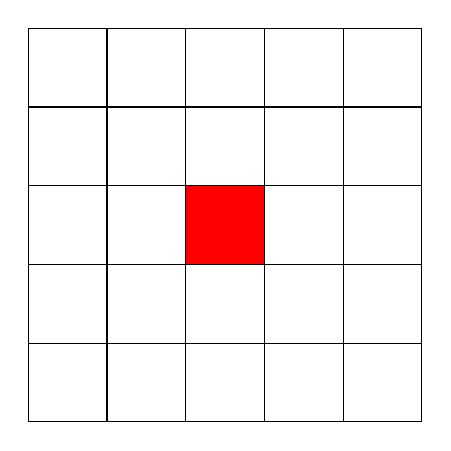
\begin{tikzpicture}
                \foreach \x in {0,1,2,3,4} {
                    \foreach \y in {0,1,2,3,4} {
                        \draw[black, thin] (\x,\y) rectangle (\x+1,\y+1);
                    }
                }
                \fill[red] (2,2) rectangle (3,3);
            \end{tikzpicture}
        } } &
        \imageWithGrid{img/qual/Perforated_Metal_3/IINet/LAM.overlay.png}{0.178\textwidth}{0.178\textwidth} &
        \imageWithGrid{img/qual/Perforated_Metal_3/DistgSSR/LAM.overlay.png}{0.178\textwidth}{0.178\textwidth} &
        \imageWithGrid{img/qual/Perforated_Metal_3/LFT/LAM.overlay.png}{0.178\textwidth}{0.178\textwidth} &
        \imageWithGrid{img/qual/Perforated_Metal_3/EPIT/LAM.overlay.png}{0.178\textwidth}{0.178\textwidth} &
        \imageWithGrid{img/qual/Perforated_Metal_3/SAT/LAM.overlay.png}{0.178\textwidth}{0.178\textwidth} \\
        % DI
        &
        DI = 9.8521 &
        DI = 9.6033 &
        DI = 7.7526 &
        DI = 5.9518 &
        DI = 27.2578 \\\hline

        \vspace{-7pt}
        \\

        % Palais_du_Luxembourg
        % Title
        % HR &
        % IINet &
        % DistgSSR &
        % LFT &
        % EPIT &
        % M2MT \\
        % main image
        \includegraphics[width=0.180\textwidth, height=0.136\textwidth]{img/qual/Palais_du_Luxembourg/HR-view.annotated.png} &
        \includegraphics[width=0.180\textwidth, height=0.136\textwidth]{img/qual/Palais_du_Luxembourg/IINet/1_3.png} &
        \includegraphics[width=0.180\textwidth, height=0.136\textwidth]{img/qual/Palais_du_Luxembourg/DistgSSR/1_3.png} &
        \includegraphics[width=0.180\textwidth, height=0.136\textwidth]{img/qual/Palais_du_Luxembourg/LFT/1_3.png} &
        \includegraphics[width=0.180\textwidth, height=0.136\textwidth]{img/qual/Palais_du_Luxembourg/EPIT/1_3.png} &
        \includegraphics[width=0.180\textwidth, height=0.136\textwidth]{img/qual/Palais_du_Luxembourg/SAT/1_3.png} \\
        % Two images
        \begin{minipage}{0.180\textwidth}
            \centering
            \includegraphics[width=0.46\textwidth, height=0.46\textwidth,cfbox=blue 1pt 0pt]{img/qual/Palais_du_Luxembourg/HR.annotated.png}
            \includegraphics[width=0.46\textwidth, height=0.46\textwidth,cfbox=red 1pt 0pt]{img/qual/Palais_du_Luxembourg/HR.LAM.png}
        \end{minipage} &
        \begin{minipage}{0.180\textwidth}
            \centering
            \includegraphics[width=0.46\textwidth, height=0.46\textwidth,cfbox=blue 1pt 0pt]{img/qual/Palais_du_Luxembourg/IINet/SR.png}
            \includegraphics[width=0.46\textwidth, height=0.46\textwidth,cfbox=red 1pt 0pt]{img/qual/Palais_du_Luxembourg/IINet/SR.LAM.png}
        \end{minipage} &
        \begin{minipage}{0.180\textwidth}
            \centering
            \includegraphics[width=0.46\textwidth, height=0.46\textwidth,cfbox=blue 1pt 0pt]{img/qual/Palais_du_Luxembourg/DistgSSR/SR.png}
            \includegraphics[width=0.46\textwidth, height=0.46\textwidth,cfbox=red 1pt 0pt]{img/qual/Palais_du_Luxembourg/DistgSSR/SR.LAM.png}
        \end{minipage} &
        \begin{minipage}{0.180\textwidth}
            \centering
            \includegraphics[width=0.46\textwidth, height=0.46\textwidth,cfbox=blue 1pt 0pt]{img/qual/Palais_du_Luxembourg/LFT/SR.png}
            \includegraphics[width=0.46\textwidth, height=0.46\textwidth,cfbox=red 1pt 0pt]{img/qual/Palais_du_Luxembourg/LFT/SR.LAM.png}
        \end{minipage} &
        \begin{minipage}{0.180\textwidth}
            \centering
            \includegraphics[width=0.46\textwidth, height=0.46\textwidth,cfbox=blue 1pt 0pt]{img/qual/Palais_du_Luxembourg/EPIT/SR.png}
            \includegraphics[width=0.46\textwidth, height=0.46\textwidth,cfbox=red 1pt 0pt]{img/qual/Palais_du_Luxembourg/EPIT/SR.LAM.png}
        \end{minipage} &
        \begin{minipage}{0.180\textwidth}
            \centering
            \includegraphics[width=0.46\textwidth, height=0.46\textwidth,cfbox=blue 1pt 0pt]{img/qual/Palais_du_Luxembourg/SAT/SR.png}
            \includegraphics[width=0.46\textwidth, height=0.46\textwidth,cfbox=red 1pt 0pt]{img/qual/Palais_du_Luxembourg/SAT/SR.LAM.png}
        \end{minipage} \\
        % PSNR/SSIM
        (b) \textit{Palais\_du\_Luxembourg} &
        18.86/\underline{0.5653} &
        18.62/0.5367 &
        18.90/0.5443 &
        \underline{18.96}/0.5584 &
        \textbf{19.68}/\textbf{0.6739} \\
        \vspace{-10pt}
        \\
        % LAM
        \raisebox{1.8\height}{
        \resizebox{0.06\textwidth}{!}{
            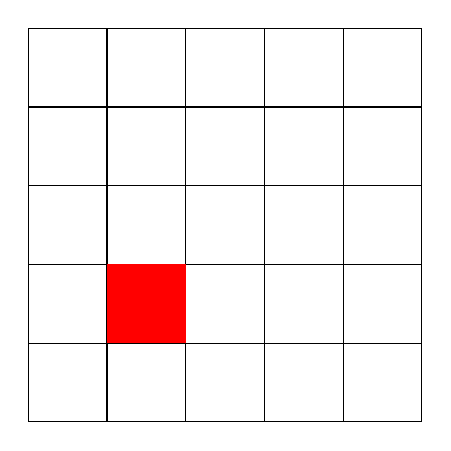
\begin{tikzpicture}
                \foreach \x in {0,1,2,3,4} {
                    \foreach \y in {0,1,2,3,4} {
                        \draw[black, thin] (\x,\y) rectangle (\x+1,\y+1);
                    }
                }
                \fill[red] (1,1) rectangle (2,2);
            \end{tikzpicture}
        } } &
        \imageWithGrid{img/qual/Palais_du_Luxembourg/IINet/LAM.overlay.png}{0.178\textwidth}{0.178\textwidth} &
        \imageWithGrid{img/qual/Palais_du_Luxembourg/DistgSSR/LAM.overlay.png}{0.178\textwidth}{0.178\textwidth} &
        \imageWithGrid{img/qual/Palais_du_Luxembourg/LFT/LAM.overlay.png}{0.178\textwidth}{0.178\textwidth} &
        \imageWithGrid{img/qual/Palais_du_Luxembourg/EPIT/LAM.overlay.png}{0.178\textwidth}{0.178\textwidth} &
        \imageWithGrid{img/qual/Palais_du_Luxembourg/SAT/LAM.overlay.png}{0.178\textwidth}{0.178\textwidth} \\
        % DI
        &
        DI = 8.0609 &
        DI = 7.8105 &
        DI = 4.1552 &
        DI = 6.5223 &
        DI = 21.0431 \\\hline

        \vspace{-7pt}
        \\

        % Bicycle
        % Title
        % HR &
        % IINet &
        % DistgSSR &
        % LFT &
        % EPIT &
        % M2MT \\
        % main image
        \includegraphics[width=0.180\textwidth, height=0.136\textwidth]{img/qual/Bicycle/HR-view.annotated.png} &
        \includegraphics[width=0.180\textwidth, height=0.136\textwidth]{img/qual/Bicycle/IINet/2_2.png} &
        \includegraphics[width=0.180\textwidth, height=0.136\textwidth]{img/qual/Bicycle/DistgSSR/2_2.png} &
        \includegraphics[width=0.180\textwidth, height=0.136\textwidth]{img/qual/Bicycle/LFT/2_2.png} &
        \includegraphics[width=0.180\textwidth, height=0.136\textwidth]{img/qual/Bicycle/EPIT/2_2.png} &
        \includegraphics[width=0.180\textwidth, height=0.136\textwidth]{img/qual/Bicycle/SAT/2_2.png} \\
        % Two images
        \begin{minipage}{0.180\textwidth}
            \centering
            \includegraphics[width=0.46\textwidth, height=0.46\textwidth,cfbox=blue 1pt 0pt]{img/qual/Bicycle/HR.annotated.png}
            \includegraphics[width=0.46\textwidth, height=0.46\textwidth,cfbox=red 1pt 0pt]{img/qual/Bicycle/HR.LAM.png}
        \end{minipage} &
        \begin{minipage}{0.180\textwidth}
            \centering
            \includegraphics[width=0.46\textwidth, height=0.46\textwidth,cfbox=blue 1pt 0pt]{img/qual/Bicycle/IINet/SR.png}
            \includegraphics[width=0.46\textwidth, height=0.46\textwidth,cfbox=red 1pt 0pt]{img/qual/Bicycle/IINet/SR.LAM.png}
        \end{minipage} &
        \begin{minipage}{0.180\textwidth}
            \centering
            \includegraphics[width=0.46\textwidth, height=0.46\textwidth,cfbox=blue 1pt 0pt]{img/qual/Bicycle/DistgSSR/SR.png}
            \includegraphics[width=0.46\textwidth, height=0.46\textwidth,cfbox=red 1pt 0pt]{img/qual/Bicycle/DistgSSR/SR.LAM.png}
        \end{minipage} &
        \begin{minipage}{0.180\textwidth}
            \centering
            \includegraphics[width=0.46\textwidth, height=0.46\textwidth,cfbox=blue 1pt 0pt]{img/qual/Bicycle/LFT/SR.png}
            \includegraphics[width=0.46\textwidth, height=0.46\textwidth,cfbox=red 1pt 0pt]{img/qual/Bicycle/LFT/SR.LAM.png}
        \end{minipage} &
        \begin{minipage}{0.180\textwidth}
            \centering
            \includegraphics[width=0.46\textwidth, height=0.46\textwidth,cfbox=blue 1pt 0pt]{img/qual/Bicycle/EPIT/SR.png}
            \includegraphics[width=0.46\textwidth, height=0.46\textwidth,cfbox=red 1pt 0pt]{img/qual/Bicycle/EPIT/SR.LAM.png}
        \end{minipage} &
        \begin{minipage}{0.180\textwidth}
            \centering
            \includegraphics[width=0.46\textwidth, height=0.46\textwidth,cfbox=blue 1pt 0pt]{img/qual/Bicycle/SAT/SR.png}
            \includegraphics[width=0.46\textwidth, height=0.46\textwidth,cfbox=red 1pt 0pt]{img/qual/Bicycle/SAT/SR.LAM.png}
        \end{minipage} \\
        % PSNR/SSIM
        (c) \textit{Bicycle} &
        27.01/0.8333 &
        26.85/0.8308 &
        27.14/0.8283 &
        \underline{27.21}/\underline{0.8367} &
        \textbf{27.37}/\textbf{0.8390} \\
        \vspace{-10pt}
        \\
        % LAM
        \raisebox{1.8\height}{
        \resizebox{0.06\textwidth}{!}{
            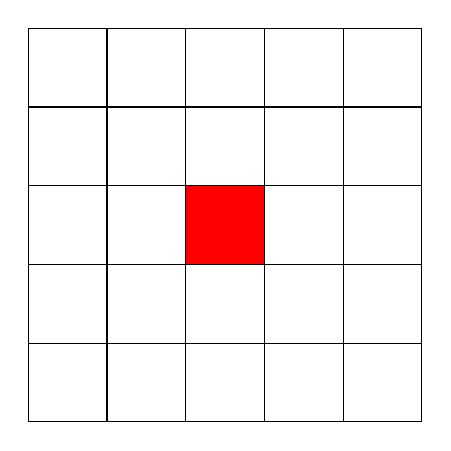
\begin{tikzpicture}
                \foreach \x in {0,1,2,3,4} {
                    \foreach \y in {0,1,2,3,4} {
                        \draw[black, thin] (\x,\y) rectangle (\x+1,\y+1);
                    }
                }
                \fill[red] (2,2) rectangle (3,3);
            \end{tikzpicture}
        } } &
        \imageWithGrid{img/qual/Bicycle/IINet/LAM.overlay.png}{0.178\textwidth}{0.178\textwidth} &
        \imageWithGrid{img/qual/Bicycle/DistgSSR/LAM.overlay.png}{0.178\textwidth}{0.178\textwidth} &
        \imageWithGrid{img/qual/Bicycle/LFT/LAM.overlay.png}{0.178\textwidth}{0.178\textwidth} &
        \imageWithGrid{img/qual/Bicycle/EPIT/LAM.overlay.png}{0.178\textwidth}{0.178\textwidth} &
        \imageWithGrid{img/qual/Bicycle/SAT/LAM.overlay.png}{0.178\textwidth}{0.178\textwidth} \\
        % DI
        &
        DI = 11.2056 &
        DI = 6.4649 &
        DI = 4.3732 &
        DI = 6.5302 &
        DI = 19.2823 \\
    \end{tabular}
    }

    \caption{Visualization of selected samples in the $4\times$ task. In each sample, the following result is provided for each compared method: the SAI, the zoom-in views from the blue and red boxes, the PSNR/SSIM of the red box, the local attribution map (LAM) of the red box and its diffusion index (DI). The best and second-best PSNR/SSIM are in bold and underlined. The angular location indicator is given below the HR.}
    \label{fig:Qual}
\end{figure*}
\begin{figure*}[ht]
    \centering
    \tabcolsep=0.05cm
    \renewcommand{\arraystretch}{1.0}
    \begin{tabular}{c}
        \includegraphics[width=0.98\textwidth]{img/qual_matrix/Perforated_Metal_3.h5.pdf} \\
        (a) \textit{Perforated\_Metal\_3} \\
        \includegraphics[width=0.98\textwidth]{img/qual_matrix/Palais_du_Luxembourg.h5.pdf} \\
        (b) \textit{Palais\_du\_Luxembourg} \\
        \includegraphics[width=0.98\textwidth]{img/qual_matrix/bicycle.h5.pdf} \\
        (c) \textit{Bicycle}
    \end{tabular}

    \caption{Visualization of SAI-wise PSNR to demonstrate the distribution of $4\times$ LFSR performance. Samples are the same with Figure \ref*{fig:Qual}.}
    \label{fig:QualMatrix}
\end{figure*}

\subsection{Angular Transformer}
With M2MT operating in the spatial subspace, an angular transformer is utilized to refine the correlations in the angular subspace. An illustration is depicted in Figure \ref{fig:M2MT}(c). This transformer is fundamentally vanilla as in \cite{liangLFT_SPL2022,wangDPT_AAAI2022}, aligning closely with Equation \ref{eq:self-attention}, but specifically operates on angular tensors $I_{A} \in \mathbb{R}^{BUV \times WH \times C}$ like Figure \ref{fig:Cubes}(c).

Notably, although the M2MT and angular Transformer operate in distinct subspaces, their primary objective converges on the establishment of a comprehensive spatial-angular representation of LF images. In subsequent experiments, we will demonstrate the synergistic benefits of their collaboration, highlighting their complementary nature.
\section{Experiments}

\subsection{Implementation Details}

In our experiments, we adhere to the protocols outlined in the commonly used BasicLFSR framework \cite{BasicLFSR} for implementing and benchmarking M2MT-Net. Five public datasets are used, namely \textit{EPFL} \cite{rerabekEPFL2016}, \textit{HCInew} \cite{honauerHCInew_ACCV2016}, \textit{HCIold} \cite{wannerHCIold_VMV2013}, \textit{INRIA} \cite{lependuINRIA_TIP2018}, and \textit{STFgantry} \cite{vaishSTFgantry_2008}. These datasets contain 70/20/10/35/9 samples for training and 10/4/2/5/2 samples for testing. Following the protocols, we only use the central $5 \times 5$ SAIs \cite{BasicLFSR}. For training, each SAI was partitioned into $64 \times 64$ or $128 \times 128$ patches to serve as HR patches, and $1/2$ or $1/4$ bicubic down-sampling is applied to produce the corresponding LR patches for $2 \times$ or $4 \times$ scales, respectively. We use Adam optimizer with a learning rate of $2 \times 10^{-4}$ and batches of 4 samples. The training process takes 100 epochs to sufficiently converge. Regarding the hyperparameters, we use $C=48$ across all Transformers and convolutions except Correlation Tensors with $C_{Cor} = 128$. The number of initial spatial convolutions is set to 4, and the number of correlation blocks $n_2$ is set to 8.

The experiments are conducted on a desktop computer with an Intel i7-11700 4.800GHz 8-core CPU, 32 MB RAM, and an Nvidia GTX 3090 GPU. We implement M2MT-Net using the PyTorch framework. The implementation code and trained models will be released publicly.

\subsection{Quantitative Comparisons}
A quantitative comparison is conducted to compare M2MT-Net with eight state-of-the-art LFSR methods on the five aforementioned datasets at $2 \times$ and $4 \times$ scales. The compared methods include convolution-based LFSSR \cite{yeungSAS_LFSR2019}, LF-ATO \cite{jinLFSSRATO_2020}, LF-InterNet \cite{wangLfInterNet_ECCV2020}, LF-IINet \cite{liuLFIINet_TMM2021}, DKNet \cite{huDKNet_TIM2022}, DistgSSR \cite{wangDistgSSR_TIP2022}, and Transformer-based methods DPT \cite{wangDPT_AAAI2022}, LFT \cite{liangLFT_SPL2022}, and EPIT \cite{liangEPIT_arXiv2023}. The outcomes are presented in Table \ref{tab:overall}.

It is evident that our M2MT-Net holds a superior position. At both the $2 \times$ and $4 \times$ scales, it achieves the highest PSNR across datasets. Notably, on the \textit{EPFL} dataset, which contains the most testing samples, M2MT-Net surpasses the second-best method, EPIT, by a significant 0.53 dB PSNR gain at the $2 \times$ scale and 0.46 dB at the $4 \times$ scale. M2MT-Net ranks second to EPIT in only one dataset, namely \textit{STFgantry}. This particular outcome can be attributed to the dataset's distinctive characteristic of exhibiting high disparities, a feature effectively managed by EPIT due to its utilization of the EPI mechanism.

A discernible trend is observed regarding the performance of Transformer-based methods on the \textit{EPFL} dataset, such as LFT and EPIT, in comparison to convolutional methods, with DistgSSR as the representative. At the $2 \times$ scale, the superiority of EPIT over DistgSSR is marginal, by just 0.02 dB, with LFT trailing further. Yet, at the $4 \times$ scale, both LFT and EPIT remarkably outdo DistgSSR by margins of 0.35 dB and 0.27 dB, respectively. This discrepancy underscores the inherent strengths of convolutions in extracting high-frequency information, particularly visual textures, which become advantageous at the $2 \times$ scale where most lost visual textures are still recoverable. Conversely, Transformers excel in modeling distant pixel or SAI dependencies, rendering them more suitable for the $4 \times$ scale where a model has to utilize existing spatial and angular cues more effectively. Different from LFT and EPIT, M2MT-Net, with the subspace isolation mitigated, integrates the advantages of both methodologies, thereby achieving significant lead margins of 0.55 dB and 0.81 dB over DistgSSR on the \textit{EPFL} dataset at both scales.

We also incorporate the geometric self-ensemble strategy, which was initially proposed for single image super-resolution \cite{limEDSR_CVPRW2017}, into M2MT-Net to enhance the model performance without introducing additional parameters. The variant is labeled as M2MT-Net* in Table \ref{tab:overall}. Similar to its application in 2D single images, during inference, the strategy transforms the 2D LR by flipping and rotating to construct an ensemble ${T_{i}\overline{I}_{LR}}$, where $T_{i}$ represents a transform function. The SR is generated by executing the network on each member in the ensemble individually, followed by the corresponding inverse transform, and finally averaging the output. The strategy is expressed as
\begin{equation}
    I_{SR} = \frac{1}{n} \sum_{i = 1}^{n} T_{i}^{-1}\mathcal{F}(T_{i}(I_{LR}))
\end{equation}
where $n$ is the number of transforms. Given that these transforms operate on the reshaped 2D SAI-view LF $\overline{I}_{LR} \in \mathbb{R}^{U V \times WH \times C}$, they take effect on both the spatial and angular spaces synergistically, ensuring the LF structure is not distorted but preserved after transform. The result in Table \ref{tab:overall} demonstrates the advantageous impact brought by the strategy with a roughly 0.10 to 0.25 dB increase in PSNR observed across the datasets and a particular 0.43 dB and 0.32 dB increase on the \textit{STFgantry} dataset at the $2 \times$ and $4 \times$ scales respectively. These findings suggest that the geometric self-ensemble strategy is a valuable addition to compensate and enhance LFSR models.


\subsection{Qualitative Comparisons}
We further explore the superior performance of LF-SANet in qualitative evaluation. Figure \ref{fig:Qual} presents qualitative results at the $4 \times$ scale for three representative samples, namely (a) \textit{Perforated\_Metal\_3}, (b) \textit{Palais\_du\_Luxembourg} and (c) \textit{Bicycle}. The first two samples are from the \textit{EPFL} dataset captured by Lytro cameras \cite{Lytro}, and the third one is from the synthetic dataset \textit{HCInew}. We compared M2MT-Net with four other methods: IINet and DistgSSR represent the convolution-based methods, while LFT and EPIT are from the Transformer-based group. Zoom-in views inside blue and red boxes are provided to show more details. Accompanying these visuals, PSNR/SSIM calculated on the red box areas. In general, all these techniques capably enhance resolution and preserve primary structures, but nuanced distinctions emerge within the details, especially the zoom-in views of red boxes.

In the \textit{Perforated\_Metal\_3} sample, most methods portray the perforated hole reasonably well but fall short in edge sharpness, likely influenced by lighting and occlusion challenges. M2MT-Net, however, produces notably sharper edges and more round shape of the hole. In the \textit{Palais\_du\_Luxembourg} sample, M2MT-Net excels in reconstructing the textures of the bricks beyond the other methods. For the \textit{Bicycle} sample, the edges of the books are clearly sharper in M2MT-Net than others.

In Figure \ref{fig:QualMatrix}, SAI-wise PSNR on these three samples is visualized. The visual representation highlights M2MT-Net's notable enhancements across SAIs. Notably, in cases (a) \textit{Perforated\_Metal\_3} and (c) \textit{Bicycle}, the lowest PSNR values achieved by M2MT-Net are still higher than the highest PSNR values of other methods. This signifies the consistent superiority of M2MT-Net.

\subsection{LAM Analysis} To further probe into the underlying capability of M2MT-Net, we employ the Local Attribution Map (LAM) technique \cite{guLAM_CVPR2021} to discern influential pixels, thereby providing insight and transparency into the performance of M2MT-Net. In Figure \ref{fig:Qual}, the LAM visualization is provided below PSNR/SSIM. It is calculated on the blue box regions with the red box regions as targets. Diffusion Index (DI) accompanies the visualization as a qualitative indicator of pixel utilization.

From the results, M2MT-Net's superior utilization across the three samples is evident, demonstrating significantly more active pixels both within and across SAIs. This superiority is further supported by the DI values as M2MT-Net consistently records values above 20, while competing methods hover at 10 or even lower. Delving deeper into these active pixels reveals intriguing insights.

For instance, in the \textit{Perforated\_Metal\_3} sample, though repeated perforated holes offer potential patterns for reconstruction, most methods focus solely on the neighboring area. In contrast, M2MT-Net's active pixels span the entire column, suggesting that it identifies shared characteristics among the holes in the column and leverages them as complementary cues. 
Similarly, in the \textit{Palais\_du\_Luxembourg} sample, the texture of brick walls exhibit recurring patterns for reuse. M2MT-Net manages to utilize not only the specific brick wall but also the neighboring one on the right, and the influential pixels have high activities across SAIs, hence the patterns are recovered with visible edges, unlike its counterparts generate a blurry area due to their narrower focus and weaker correlation across SAIs.
For the \textit{Bicycle} sample, the books on the shelves present similar patterns as well. M2MT-Net's advantage becomes evident as it activates pixels not only around the local area but also on a book in a similar red color on the shelf above, regardless of the distance.

The DI values offer insights into the relationship between model performance and pixel utilization. In theory, higher DI indicates better pixel utilization and should result in improved performance. This holds true for M2MT-Net, as it achieves a double-digit DI alongside significantly higher PSNR and SSIM scores, and it still holds true if comparing only within the convolution-based or Transformer-based groups.

The DI values shed light on the relation between model performance and pixel utilization. In theory, higher DI indicates higher pixel utilization and should result in better performance. It holds true for M2MT-Net as having a double-digit DI and a significantly higher PSNR and SSIM, and it remains consistent when comparing only within the convolution-based or Transformer-based groups. However, when comparing across these two groups, a different trend emerges as convolution-based IINet and DistgSSR tend to have higher DI values but often lag behind Transformer-based LFT and EPIT in terms of PSNR and SSIM. This highlights the distinct nature of pixel utilization between convolutions and Transformers, where convolutions leverage more pixels but are constrained by locality, while Transformers use fewer pixels in a more effective way through its global dependency modeling mechanism.

\begin{figure*}[ht!]
    \centering
    \tabcolsep=0.05cm
    \renewcommand{\arraystretch}{1.0}
    {\small 
    \begin{tabular}{ccccccc}
    % Perforated_Metal_3
    \raisebox{-0.5\height}[0pt][0pt]{
        \includegraphics[width=0.25\textwidth, height=0.17\textwidth]{img/depth/full/Perforated_Metal_3/rgb_annotated.png}
    } &
    \includegraphics[width=0.110\textwidth, height=0.110\textwidth,cfbox=blue 1pt 0pt]{img/depth/crop/Perforated_Metal_3/GT_1.png} &
    \includegraphics[width=0.110\textwidth, height=0.110\textwidth,cfbox=blue 1pt 0pt]{img/depth/crop/Perforated_Metal_3/IINet_1.png} &
    \includegraphics[width=0.110\textwidth, height=0.110\textwidth,cfbox=blue 1pt 0pt]{img/depth/crop/Perforated_Metal_3/DistgSSR_1.png} &
    \includegraphics[width=0.110\textwidth, height=0.110\textwidth,cfbox=blue 1pt 0pt]{img/depth/crop/Perforated_Metal_3/LFT_1.png} &
    \includegraphics[width=0.110\textwidth, height=0.110\textwidth,cfbox=blue 1pt 0pt]{img/depth/crop/Perforated_Metal_3/EPIT_1.png} &
    \includegraphics[width=0.110\textwidth, height=0.110\textwidth,cfbox=blue 1pt 0pt]{img/depth/crop/Perforated_Metal_3/SATNet_1.png} \\
    &
    \includegraphics[width=0.110\textwidth, height=0.110\textwidth,cfbox=red 1pt 0pt]{img/depth/crop/Perforated_Metal_3/GT_2.png} &
    \includegraphics[width=0.110\textwidth, height=0.110\textwidth,cfbox=red 1pt 0pt]{img/depth/crop/Perforated_Metal_3/IINet_2.png} &
    \includegraphics[width=0.110\textwidth, height=0.110\textwidth,cfbox=red 1pt 0pt]{img/depth/crop/Perforated_Metal_3/DistgSSR_2.png} &
    \includegraphics[width=0.110\textwidth, height=0.110\textwidth,cfbox=red 1pt 0pt]{img/depth/crop/Perforated_Metal_3/LFT_2.png} &
    \includegraphics[width=0.110\textwidth, height=0.110\textwidth,cfbox=red 1pt 0pt]{img/depth/crop/Perforated_Metal_3/EPIT_2.png} &
    \includegraphics[width=0.110\textwidth, height=0.110\textwidth,cfbox=red 1pt 0pt]{img/depth/crop/Perforated_Metal_3/SATNet_2.png} \\
    
    \textit{Perforated\_Metal\_3} &
    Ground-truth &
    IINet \cite{liuLFIINet_TMM2021} &
    DistgSSR \cite{wangDistgSSR_TIP2022} &
    LFT \cite{liangLFT_SPL2022} &
    EPIT \cite{liangEPIT_arXiv2023} &
    M2MT-Net \\

    MSE$\times100$ &
    &
    0.968 &
    \underline{0.832} &
    1.037 &
    0.918 &
    \textbf{0.706} \\

    \vspace{-5pt} \\

    % Sphynx
    \raisebox{-0.5\height}[0pt][0pt]{
        \includegraphics[width=0.25\textwidth, height=0.17\textwidth]{img/depth/full/Sphynx/rgb_annotated.png}
    } &
    \includegraphics[width=0.110\textwidth, height=0.110\textwidth,cfbox=blue 1pt 0pt]{img/depth/crop/Sphynx/GT_1.png} &
    \includegraphics[width=0.110\textwidth, height=0.110\textwidth,cfbox=blue 1pt 0pt]{img/depth/crop/Sphynx/IINet_1.png} &
    \includegraphics[width=0.110\textwidth, height=0.110\textwidth,cfbox=blue 1pt 0pt]{img/depth/crop/Sphynx/DistgSSR_1.png} &
    \includegraphics[width=0.110\textwidth, height=0.110\textwidth,cfbox=blue 1pt 0pt]{img/depth/crop/Sphynx/LFT_1.png} &
    \includegraphics[width=0.110\textwidth, height=0.110\textwidth,cfbox=blue 1pt 0pt]{img/depth/crop/Sphynx/EPIT_1.png} &
    \includegraphics[width=0.110\textwidth, height=0.110\textwidth,cfbox=blue 1pt 0pt]{img/depth/crop/Sphynx/SATNet_1.png} \\
    &
    \includegraphics[width=0.110\textwidth, height=0.110\textwidth,cfbox=red 1pt 0pt]{img/depth/crop/Sphynx/GT_2.png} &
    \includegraphics[width=0.110\textwidth, height=0.110\textwidth,cfbox=red 1pt 0pt]{img/depth/crop/Sphynx/IINet_2.png} &
    \includegraphics[width=0.110\textwidth, height=0.110\textwidth,cfbox=red 1pt 0pt]{img/depth/crop/Sphynx/DistgSSR_2.png} &
    \includegraphics[width=0.110\textwidth, height=0.110\textwidth,cfbox=red 1pt 0pt]{img/depth/crop/Sphynx/LFT_2.png} &
    \includegraphics[width=0.110\textwidth, height=0.110\textwidth,cfbox=red 1pt 0pt]{img/depth/crop/Sphynx/EPIT_2.png} &
    \includegraphics[width=0.110\textwidth, height=0.110\textwidth,cfbox=red 1pt 0pt]{img/depth/crop/Sphynx/SATNet_2.png} \\
    
    \textit{Sphynx} &
    Ground-truth &
    IINet \cite{liuLFIINet_TMM2021} &
    DistgSSR \cite{wangDistgSSR_TIP2022} &
    LFT \cite{liangLFT_SPL2022} &
    EPIT \cite{liangEPIT_arXiv2023} &
    M2MT-Net \\

    MSE$\times100$ &
    &
    0.178 &
    \underline{0.139} &
    0.149 &
    0.147 &
    \textbf{0.136} \\

    \vspace{-5pt} \\

    % bicycle
    \raisebox{-0.5\height}[0pt][0pt]{
        \includegraphics[width=0.22\textwidth, height=0.22\textwidth]{img/depth/full/bicycle/rgb_annotated.png}
    } &
    \includegraphics[width=0.110\textwidth, height=0.110\textwidth,cfbox=blue 1pt 0pt]{img/depth/crop/bicycle/GT_1.png} &
    \includegraphics[width=0.110\textwidth, height=0.110\textwidth,cfbox=blue 1pt 0pt]{img/depth/crop/bicycle/IINet_1.png} &
    \includegraphics[width=0.110\textwidth, height=0.110\textwidth,cfbox=blue 1pt 0pt]{img/depth/crop/bicycle/DistgSSR_1.png} &
    \includegraphics[width=0.110\textwidth, height=0.110\textwidth,cfbox=blue 1pt 0pt]{img/depth/crop/bicycle/LFT_1.png} &
    \includegraphics[width=0.110\textwidth, height=0.110\textwidth,cfbox=blue 1pt 0pt]{img/depth/crop/bicycle/EPIT_1.png} &
    \includegraphics[width=0.110\textwidth, height=0.110\textwidth,cfbox=blue 1pt 0pt]{img/depth/crop/bicycle/SATNet_1.png} \\
    &
    \includegraphics[width=0.110\textwidth, height=0.110\textwidth,cfbox=red 1pt 0pt]{img/depth/crop/bicycle/GT_2.png} &
    \includegraphics[width=0.110\textwidth, height=0.110\textwidth,cfbox=red 1pt 0pt]{img/depth/crop/bicycle/IINet_2.png} &
    \includegraphics[width=0.110\textwidth, height=0.110\textwidth,cfbox=red 1pt 0pt]{img/depth/crop/bicycle/DistgSSR_2.png} &
    \includegraphics[width=0.110\textwidth, height=0.110\textwidth,cfbox=red 1pt 0pt]{img/depth/crop/bicycle/LFT_2.png} &
    \includegraphics[width=0.110\textwidth, height=0.110\textwidth,cfbox=red 1pt 0pt]{img/depth/crop/bicycle/EPIT_2.png} &
    \includegraphics[width=0.110\textwidth, height=0.110\textwidth,cfbox=red 1pt 0pt]{img/depth/crop/bicycle/SATNet_2.png} \\
    
    \textit{bicycle} &
    Ground-truth &
    \small IINet \cite{liuLFIINet_TMM2021} &
    DistgSSR \cite{wangDistgSSR_TIP2022} &
    LFT \cite{liangLFT_SPL2022} &
    EPIT \cite{liangEPIT_arXiv2023} &
    M2MT-Net \\

    MSE$\times100$ &
    &
    2.805 &
    2.633 &
    2.652 &
    \underline{2.557} &
    \textbf{2.324} \\

    \vspace{-5pt} \\

    % monasRoom
    \raisebox{-0.5\height}[0pt][0pt]{
        \includegraphics[width=0.22\textwidth, height=0.22\textwidth]{img/depth/full/monasRoom/rgb_annotated.png}
    } &
    \includegraphics[width=0.110\textwidth, height=0.110\textwidth,cfbox=blue 1pt 0pt]{img/depth/crop/monasRoom/GT_1.png} &
    \includegraphics[width=0.110\textwidth, height=0.110\textwidth,cfbox=blue 1pt 0pt]{img/depth/crop/monasRoom/IINet_1.png} &
    \includegraphics[width=0.110\textwidth, height=0.110\textwidth,cfbox=blue 1pt 0pt]{img/depth/crop/monasRoom/DistgSSR_1.png} &
    \includegraphics[width=0.110\textwidth, height=0.110\textwidth,cfbox=blue 1pt 0pt]{img/depth/crop/monasRoom/LFT_1.png} &
    \includegraphics[width=0.110\textwidth, height=0.110\textwidth,cfbox=blue 1pt 0pt]{img/depth/crop/monasRoom/EPIT_1.png} &
    \includegraphics[width=0.110\textwidth, height=0.110\textwidth,cfbox=blue 1pt 0pt]{img/depth/crop/monasRoom/SATNet_1.png} \\
    &
    \includegraphics[width=0.110\textwidth, height=0.110\textwidth,cfbox=red 1pt 0pt]{img/depth/crop/monasRoom/GT_2.png} &
    \includegraphics[width=0.110\textwidth, height=0.110\textwidth,cfbox=red 1pt 0pt]{img/depth/crop/monasRoom/IINet_2.png} &
    \includegraphics[width=0.110\textwidth, height=0.110\textwidth,cfbox=red 1pt 0pt]{img/depth/crop/monasRoom/DistgSSR_2.png} &
    \includegraphics[width=0.110\textwidth, height=0.110\textwidth,cfbox=red 1pt 0pt]{img/depth/crop/monasRoom/LFT_2.png} &
    \includegraphics[width=0.110\textwidth, height=0.110\textwidth,cfbox=red 1pt 0pt]{img/depth/crop/monasRoom/EPIT_2.png} &
    \includegraphics[width=0.110\textwidth, height=0.110\textwidth,cfbox=red 1pt 0pt]{img/depth/crop/monasRoom/SATNet_2.png} \\
    
    \textit{monasRoom} &
    Ground-truth &
    IINet \cite{liuLFIINet_TMM2021} &
    DistgSSR \cite{wangDistgSSR_TIP2022} &
    LFT \cite{liangLFT_SPL2022} &
    EPIT \cite{liangEPIT_arXiv2023} &
    M2MT-Net \\

    MSE$\times100$ &
    &
    0.584 &
    0.571 &
    0.590 &
    \underline{0.567} &
    \textbf{0.560} \\

    \end{tabular}
    }
    \caption{Visualization of depth estimation on the $4\times$ LFSR results of our M2MT-Net and the current state-of-the-art methods. Zoom-in depth maps are depicted on the areas in the blue and red boxes. MSE$\times 100$ is evaluated on the entire depth map. The best and second-best MSE are in bold and underlined.}
    \label{fig:Depth}
\end{figure*}
    

\subsection{Angular Consistency}
While the reconstruction of visual detail is important for LFSR, the preservation of parallax structure within LF images is equally crucial. This aspect of parallax structure cannot be adequately discerned solely by examining the reconstructed SAIs. Thus, to comprehensively assess the angular consistency, we conduct an evaluation through depth estimation. OACC-Net \cite{wangOACCNet_CVPR2022} is applied to generate depth maps on the super-resolved output of the methods under comparison. The depth estimated from HR images serves as the ground truth for this evaluation. Figure \ref{fig:Depth} visually represents the depth maps for two real-world and synthetic examples, accompanied by the $MSE\times100$ as a quantitative evaluation metric.

M2MT-Net's superiority, as highlighted in \textit{Perforated\_Metal\_3} of Figure \ref{fig:Qual}, is corroborated in the generated depth map. This method successfully reconstructs perforated holes with crisply integrated edges spanning from near to distant from the camera as evidenced in the blue and red boxes. In stark contrast, competing methods struggle, yielding blurred and entangled edges in this complex scene. When examining scenes featuring salient objects, M2MT-Net continues to excel. In the \textit{Sphynx} sample, the contours of the sphynx's nose, mouth and neck are distinctly delineated in M2MT-Net's depth map. Other methods, however, generate noticeable blurs or artifacts in these areas. The \textit{bicycle} sample further illustrates M2MT-Net's proficiency, where distinct separations between the bicycle's handlebar and the background are evident, as well as more continuous structures in the plant's trunks. Other methods falter, blending the handlebar's contour with the background or breaking the trunk's structure into fragments. Finally, in the \textit{monasRoom} example, M2MT-Net's depth map reveals a smoother surface on the T-shaped object and sharper contours on the leaf with fewer inaccuracies, demonstrating a closer approximation to the ground-truth when compared to the other methods, which produce noticeable bumpy artifacts.

These results collectively underscore M2MT-Net's leading capability not only in reconstructing visual details but also in preserving the parallax structure in super-resolved LF images, marking it as a significant advancement in LFSR.

\begin{table}[ht]
    \centering
    \caption{Comparison of computational efficiency against the state-of-the-art methods at the $4 \times$ scale. Runtime is the average elapsed time per sample over all 23 samples. \#Params is the number of trainable parameters.}
    \label{tab:efficiency}
    
    \begin{tabular}{|c|c|c|c|}
    \hline

    Method                                  & Type                  & Runtime/s   & \#Params   \\ \hline
    LF-IINet \cite{liuLFIINet_TMM2021}      & Convolution-based     & 1.34        & 4,885,824 \\
    DistgSSR \cite{wangDistgSSR_TIP2022}    & Convolution-based     & 1.70        & 3,581,568 \\
    LFT \cite{liangLFT_SPL2022}             & Transformer-based     & 5.84        & 1,163,392 \\
    EPIT \cite{liangEPIT_arXiv2023}         & Transformer-based     & 3.16        & 1,470,080 \\
    M2MT (Ours)                             & Transformer-based     & 2.03        & 3,986,400 \\
    \hline
    
    \end{tabular}
\end{table}
\begin{figure}[ht]
    \centering
    \tabcolsep=0.01cm
    \renewcommand{\arraystretch}{0.8}
    \begin{tabular}{c}
        \includegraphics[width=0.35\textwidth]{img/tradeoff/runtime.pdf} \\
        (a) PSNR vs Runtime \\
        \includegraphics[width=0.35\textwidth]{img/tradeoff/parameter.pdf} \\
        (b) PSNR vs Parameter Number
    \end{tabular}
    \caption{Tradeoff between performance and efficiency at the $4\times$ scale. The convolution-based methods are in red while the Transformer-based methods are in green. Candidates positioned closer to the top-right corner of the plots are better. }
    \label{fig:tradeoff}
\end{figure}


\subsection{Computational Efficiency}
We evaluate the computational efficiency of M2MT-Net against the best competitors LF-IINet, DistgSSR, LFT, and EPIT. Two metrics are involved: the running speed and the number of trainable parameters. The running speed measures the elapsed time per sample when running all 23 samples. The result is shown in Table \ref{tab:efficiency}, and the tradeoff between PSNR and runtime/parameter numbers is visualized as plots in Figure \ref{fig:tradeoff}. The convolution-based methods are in red while the Transformer-based methods are in green. In general, candidates positioned closer to the top-right corner of the plots indicate a more favorable tradeoff between performance and efficiency.

In terms of runtime, LF-IINet and DistgSSR are the fastest method as its convolution operations are local, making it quicker than global Transformer operations. Yet, within Transformer-based techniques, M2MT-Net emerges as the swiftest, taking approximately 20\% more time than DistgSSR but being 35\% and 65\% faster than EPIT and LFT respectively. This advantage is attributed to M2MT reducing the channel dimension from $UVC$ to $C_{Cor}$ via its linear layer in correlation encoding, significantly trimming the computational demand of the following self-attention component. On the flip side, this channel conversion makes M2MT bulkier in model size, as the linear layers require more parameters in both correlation encoding and decoding. Still, LF-SANet has 19\% fewer parameters than LF-IINet and 11\% more parameters than DistgSSR, keeping its size fairly manageable.

\subsection{Ablation Study}
In this section, we undertake a few ablation studies to understand the characteristic of M2MT-Net and its individual components. Note that the studies are carried out at the most challenging $4 \times$ scale using the \textit{EPFL} dataset as it has the most samples.

\subsubsection{Spatial and Angular Components}
To evaluate our proposed M2MT's role in the spatial subspace, we substitute it with a vanilla Transformer or a convolution and trained the network. The modified networks have similar sizes with the original M2MT-Net to ensure a fair comparison. As indicated in Table \ref{tab:ablation_altering}, substituting the M2MT with a vanilla Transformer deteriorates the performance by 0.51 dB to 29.29 dB. Opting for a convolution results in a further decline, with a drop of 0.78 dB to 29.02 dB. These outcomes affirm M2MT's efficacy as a feature extractor in the spatial subspace than other alternatives when paired with its angular subspace counterpart.

We also train a model replacing the angular Transformer with a convolution. Surprisingly, this variant achieves 29.42 dB PSNR, slightly outperforming Transformer-based competitors like LFT and EPIT. This underscores the robust adaptability of the M2MT, even when paired with less potent components.

\subsubsection{Number of Correlation Blocks}
We explore the performance of M2MT-Net with varying the number of correlation blocks $n_2$. Table \ref{tab:ablation_number_blocks} shows that M2MT-Net peaks in performance at $n_2 = 8$. Reducing the number leads to a gradual performance decline, and increasing it doesn't guarantee performance improvement due to the potential risk of overfitting.

\begin{table}[t!]
    \centering
    %\scriptsize
    \caption{Ablation study on altering components in correlation blocks. The best PSNR/SSIM are in bold.}
    \label{tab:ablation_altering}
    \resizebox{.45\textwidth}{!}{
    \begin{tabular}{|c|c|c|}
    \hline

    Spatial Component   &   Angular Component   & PSNR/SSIM \\ \hline
    M2MT                &   Vanilla Transformer & \textbf{29.80}/\textbf{0.9277} \\
    Vanilla Transformer &   Vanilla Transformer & 29.29/0.9213 \\
    Convolution         &   Vanilla Transformer & 29.02/0.9199 \\
    M2MT                &   Convolution         & 29.42/0.9208 \\
    % Convolution         &   Convolution         & 28.77/0.9135 \\
    \hline
    \end{tabular}
    }
\end{table}
\begin{table}[t!]
    \centering
    \caption{Ablation study on varing the number of correlation blocks. The best PSNR/SSIM are in bold.}
    \label{tab:ablation_number_blocks}
    \resizebox{.45\textwidth}{!}{
    \begin{tabular}{|c|c|c|c|c|c|}
    \hline

    % Number    & PSNR/SSIM \\ \hline
    % 6         & 29.49/0.9233 \\
    % 7         & 29.58/0.9239 \\
    % 8         & \textbf{29.67}/\textbf{0.9247} \\
    % 9         & 29.54/0.9223 \\
    % 10        & 29.60/\textbf{0.9247} \\

    Number    & 6       & 7         & 8                 & 9         & 10        \\ \hline
    PSNR      & 29.60   & 29.69     & \textbf{29.80}    & 29.65     & 29.66     \\
    SSIM      & 0.9257  & 0.9270    & \textbf{0.9277}   & 0.9270    & 0.9271    \\
    \hline
    
    \end{tabular}
    }
\end{table}
\section{Conclusion}
In this paper, we have revealed the prevalent challenge of subspace isolation caused by the One-to-One scheme and present the novel concept of Many-to-Many Transformers (M2MT) as a new scheme to address this issue. The proposed M2MT is empowered with complete access to all pixels across all SAIs in a LF image to capture comprehensive long-range correlation dependencies. With M2MT as a pivotal component, we have proposed a simple yet effective M2MT-Net for LFSR. Extensive experiments on various public datasets have demonstrated that M2MT-Net surpasses state-of-the-art methods to a considerable extent. Its superiority is evidenced by visual interpretability in our in-depth analysis using the LAM technique, which highlights that M2MT involves a substantially broader range of pixels across wider SAIs beyond subspace isolation, signifying its truly global context and a more comprehensive modeling of correlation dependencies.

Looking ahead, there are some promising directions for improving M2MT in future works. Firstly, extending M2MT to EPI subspaces could potentially reinforce M2MT's capacity to process LF images with large disparities like the \textit{STFgantry} dataset \cite{vaishSTFgantry_2008}, akin to EPIT \cite{liangEPIT_arXiv2023}. However, the unique characteristics of EPIs present distinct challenges that necessitate further investigation. Secondly, M2MT-Net currently carries a relatively substantial model size when compared to other Transformer-based methods, despite its commendable speed. This is primarily attributed to the correlation encoding and decoding processes within M2MT. It would be advantageous to explore lightweight alternatives to achieve a balanced trade-off between computational efficiency and performance in future research endeavors.

\bibliographystyle{IEEEtran}
\bibliography{reference}

\end{document}


